% \iffalse meta-comment
%
% Copyright (C) 2007 by Matthew Allen
% 
% ---------------------------------------------
% This file is part of the newspaper package,
% a contribution to the LaTeX2e system.
% ---------------------------------------------
%
% It may be distributed and/or modified under the conditions of the
% LaTeX Project Public License. The latest version of this license is at
% http://www.latex-project.org/lppl.txt 
%
%
% \fi
% 
% \iffalse
%<package>\ProvidesPackage{newspaper}
%<package>\NeedsTexFormat{LaTeX2e}
%
%<*driver>
\documentclass{ltxdoc}
\usepackage[pdftex]{graphicx}
\usepackage{pdflscape} % begin{landscape}
\DisableCrossrefs %Disables indexing of code (to enable ->\EnableCrossrefs)
\CodelineIndex
\RecordChanges
\begin{document}
	\DocInput{newspaper.dtx}
\end{document}
%</driver>
%
% \fi
%
% \CheckSum{0}
%
% \CharacterTable
%  {Upper-case    \A\B\C\D\E\F\G\H\I\J\K\L\M\N\O\P\Q\R\S\T\U\V\W\X\Y\Z
%   Lower-case    \a\b\c\d\e\f\g\h\i\j\k\l\m\n\o\p\q\r\s\t\u\v\w\x\y\z
%   Digits        \0\1\2\3\4\5\6\7\8\9
%   Exclamation   \!     Double quote  \"     Hash (number) \#
%   Dollar        \$     Percent       \%     Ampersand     \&
%   Acute accent  \'     Left paren    \(     Right paren   \)
%   Asterisk      \*     Plus          \+     Comma         \,
%   Minus         \-     Point         \.     Solidus       \/
%   Colon         \:     Semicolon     \;     Less than     \<
%   Equals        \=     Greater than  \>     Question mark \?
%   Commercial at \@     Left bracket  \[     Backslash     \\
%   Right bracket \]     Circumflex    \^     Underscore    \_
%   Grave accent  \`     Left brace    \{     Vertical bar  \|
%   Right brace   \}     Tilde         \~}
%
% \changes{v1.0}{2007/06/12}{initial version}
% 
% \GetFileInfo{newspaper.sty}
%
% \DoNotIndex{\#,\$} 
% 
% \title{The \textsf{newspaper} Package}
% \author{Matthew Allen}
% \date{\today}
%
% \maketitle
% 
% \begin{abstract}
%  	The \textsf{newspaper} package redefines the page style and |\maketitle| command to 
%		produce a typeset page similar to that off a newspaper.  It also provides several 
%		commands that (when used with other packages) allow the ease of writing articles
%		in a newspaper-style column format. 
% \end{abstract}
%
% \section{Introduction}
% In the early part of 2007, the lab where I was working sent me off to Washington to be a staffer at the House of Representatives.  So the lab wouldn't forget about me -- and also to keep up my \LaTeX\ skills -- I decided to send back a newsletter once a month.  To my great surprise, I couldn't find a suitable \LaTeX\ package for typesetting a newsletter.  Therefore, I set about to write the package myself.  The \textsf{newspaper} package is the result of this effort.     
%
% This package is a very simple package that redefines the page style and |\maketitle| command to produce a typeset page similar to that off a newspaper.  It also provides several commands that (when used with other packages) allow the ease of writing articles in a newspaper-style column format.  The result of the |\maketitle| command is shown in Figure~\ref{fig:heading}.  As you can see from the figure, the style is based on that of the \emph{New York Times}.  Commands for redefining the default values for Title, Date, and Slogan are described in the sections below. 
% \begin{figure}[t]
% 
\includegraphics[width=\textwidth]{Figure1}
% \caption{Default heading acquired with the \textsf{newspaper} package.}
% \label{fig:heading}
% \end{figure}
%	
%	\section{Requirements}
%	This system requires both \LaTeXe\ and the \textsf{yfonts} package developed by Walter Schmidt.  
%	The package itself is never actually loaded, but the |ygoth| font is called and used to typeset the heading.
%	These are the only \emph{required} packages.  However, several additional packages (e.g. \textsf{multicols} by
%	Frank Mittelbach	and	\textsf{picinpar} by Friedhlem Sowa) enhance the use of the \textsf{newspaper} package.  				%	Examples of these additional packages
%	are discussed in Section~\ref{additionalpackages}.
% 
% \section{User Interface}
%	When loaded \textsf{newspaper} sets up a number of defaults (detailed later).  These defaults can be modified by specific commands.
%	Load the package in the usual way as
%	\begin{quote}
%	|\usepackage{newspaper}|
%	\end{quote}
%	which immediately redefines the page style on the first page to resemble that of a newspaper, 
%	as shown in Figure~\ref{fig:heading}.
%	It also redefines the page style on all subsequent pages to provide the appropriate title, date, and 
%	page number.
%
%	There are three commands that must be set in the preamble of the document.  That is, they must
%	be defined before the |\begin{document}| command.
%	These commands are:
%	\begin{quote}
%	|\date|\marg{date}\\
%	|\currentvolume|\marg{real}\\
%	|\currentissue|\marg{real}\\
%	\end{quote}
%	where \marg{date} is the date (which could be |\today|), and \marg{real} is any real number.
%	The volume number is set in Roman numerals and the issue number is set in arabic numerals as shown
%	on the left side of Figure~\ref{fig:heading}.
%	
% \subsection{Default Behaviour and Commands to Modify It}
%	The default parameters of the \textsf{newspaper} package are shown in Table~\ref{tab:packagedefaults}.
%	Without actually specifying any changes, these settings will produce the output shown in Figure~\ref{fig:heading}.
%	
%	You'll notice there are two parameters that contain a similar setting: Paper Name and Header Name.
%	This is necessary because the first page has a different heading page style than all subsequent pages.
%	On this first page, the heading is that shown in Figure~\ref{fig:heading}, in which the Paper Name is set with \emph{gothic} 	font.  In this font some letters appear different
%	from modern type.  Specifically	the modern \emph{s} is defined specifically by adding the colon.  
%	If that isn't done, the gothic \emph{s}	is used, which looks more like the modern \emph{f} than the modern \emph{s}.  
%
%	All subsequent pages have a different heading that is comprised of the Header Name which is supposedly the same as the 			Paper Name but set in whatever font is used for the main text.  If we used just one parameter (say the Paper Name) we would 	run the risk of having colons appear after characters in the heading on subsequent pages.  
%	
%	\begin{table}[htb]
%	\begin{center}
%		\DeleteShortVerb{\|}
%		\begin{tabular}{|p{1.25in}p{1.75in}|}
%			\hline
%			\MakeShortVerb{\|}
%			Parameter				&	Default Value\\
%			\hline\hline
%			Paper Name 			& Committee Times:\\
%			Header Name			& Committee Times\\
%			Paper Location	& Washington DC\\
%			Paper Slogan		& ``All the news\dots''\\
%			Paper Price			& Zero Dollars\\
%			\hline
%		\end{tabular}
%	\end{center}
%	\caption{Package Defaults}
%	\label{tab:packagedefaults}
%	\end{table}
%	
%	If you would like to customize the parameters, the appropriate commands are shown in Table~\ref{tab:packagebehaviour}.
%	For example, to change the title of the paper simply add a line in the preamble that contains
%	|\SetPaperName{My Title}|.  Remember, to change the header name appropriately (in this case by adding
%	|\SetHeaderName{My Title}|.  
%
%	\begin{table}[htb]
%	\begin{center}
%		\DeleteShortVerb{\|}
%		\begin{tabular}{|p{1.25in}p{2.0in}|}
%			\hline
%			\MakeShortVerb{\|}
%			Parameter				&	Command to Change Parameter\\
%			\hline\hline
%			Paper Name 			& |\SetPaperName|\marg{text}\\
%			Header Name			& |\SetHeaderName|\marg{text}\\
%			Paper Location	& |\SetPaperLocation|\marg{text}\\
%			Paper Slogan		& |\SetPaperSlogan|\marg{text}\\
%			Paper Price			& |\SetPaperPrice|\marg{text}\\
%			\hline
%		\end{tabular}
%	\end{center}
%	\caption{The necessary commands to affect package behaviour.}
%	\label{tab:packagebehaviour}
%	\end{table}
% 
% \subsection{Additional Suggested Packages}
%	\label{additionalpackages}
% The use of additional packages will greatly enhance the appearance of any ``newspaper'' style document.
%	First and foremost, the \textsf{multicols} package by Frank Mittelbach is by the far the best means of
%	producing columns of text.  Unlike the |\twocoloum| command available to \LaTeX,\ the \textsf{multicols}
%	package makes it possible to go between one coloum, two coloums, and three columns of text on the \emph{same} page.
%	
%	Two other very useful packages are the \textsf{picinpar} package by Friedhelm Sowa and the \textsf{hyperref} package
%	by Sebastian Rahtz.  The \textsf{picinpar} package provides several useful commands for creating empty rectangular
%	spaces within a block of text.  This is especially useful for setting figures in columns of text -- especially
%	since the \textsf{multicols} package does not allow the use of floats inside columns.
%	
%	The \textsf{hyperref} package is always a good idea when the final format is a PDF file.  The package provides a wealth
%	of commands that enable hyperlinks, and govern how the file is opened and displayed.  For example, when I was sending
%	my newsletters back to the home office, I had a self-imposed maximum-length constraint of two pages.  Keeping a newsletter short is one way to increase the number of people that will actually read it.  
%	Loading the \textsf{hyperref} package with the options
%	\begin{quote}
%	|\usepackage[pdfpagemode={none},|\\
%	\hspace*{1in}|pdfpagelayout={TwoColumnRight}]{hyperref}|
%	\end{quote}
%	ensured the resulting PDF file opened with bookmarks closed and in two-page display mode.
%
%	One other package I found very useful was the \textsf{Times} package.  It's a small package, in fact
%	the entire contents of the package is only three lines of code:
%	\begin{quote}
%	|\renewcommand{\sfdefault}{phv}| \\
%	|\renewcommand{\rmdefault}{ptm}|\\
%	|\renewcommand{\ttdefault}{pcr}|
%	\end{quote}
%	The package changes \TeX's default San Serif, Roman, and Type Writer fonts to Helvetica, Times-Roman, and Courier
%	respectively.
%	
%	As a general rule, Times-Roman (or Times New Roman as its variants are sometimes called) is a terrible font and should 	always be	avoided.  There is, however, one exception to the rule: when setting columns of text.  The Times New Roman typeface was developed in 1931 for \emph{The Times} of London.  The letters are more narrow than other typefaces and the ascenders and
%	descenders are smaller.  This makes it ideal for newspapers, that always strive to squeeze more words onto a single
%	page 
%	in order to reduce production costs.  Its economic advatage has made it popular with book publishers in the United
%	States.  
%
%	The ability to squeeze more words onto a page is advantagous if you have a maximum length constraint of two pages, as
%	I did for my newsletters.  Even though the letters are narrow, reading short columns of text is easier on the eyes than
%	moving your eyes back and forth across the length of an entire page.  
%	Such a font should never be used to set large pages of text because it will fatigue the eyes of the reader.
%
%	An example of using the \textsf{newspaper} package in combination with the packages mentioned above is shown in
%	Figure~\ref{fig:example}.   
%	
% \begin{landscape}
%	\begin{figure}[t]
%	\begin{center}
% \rotatebox{-90}{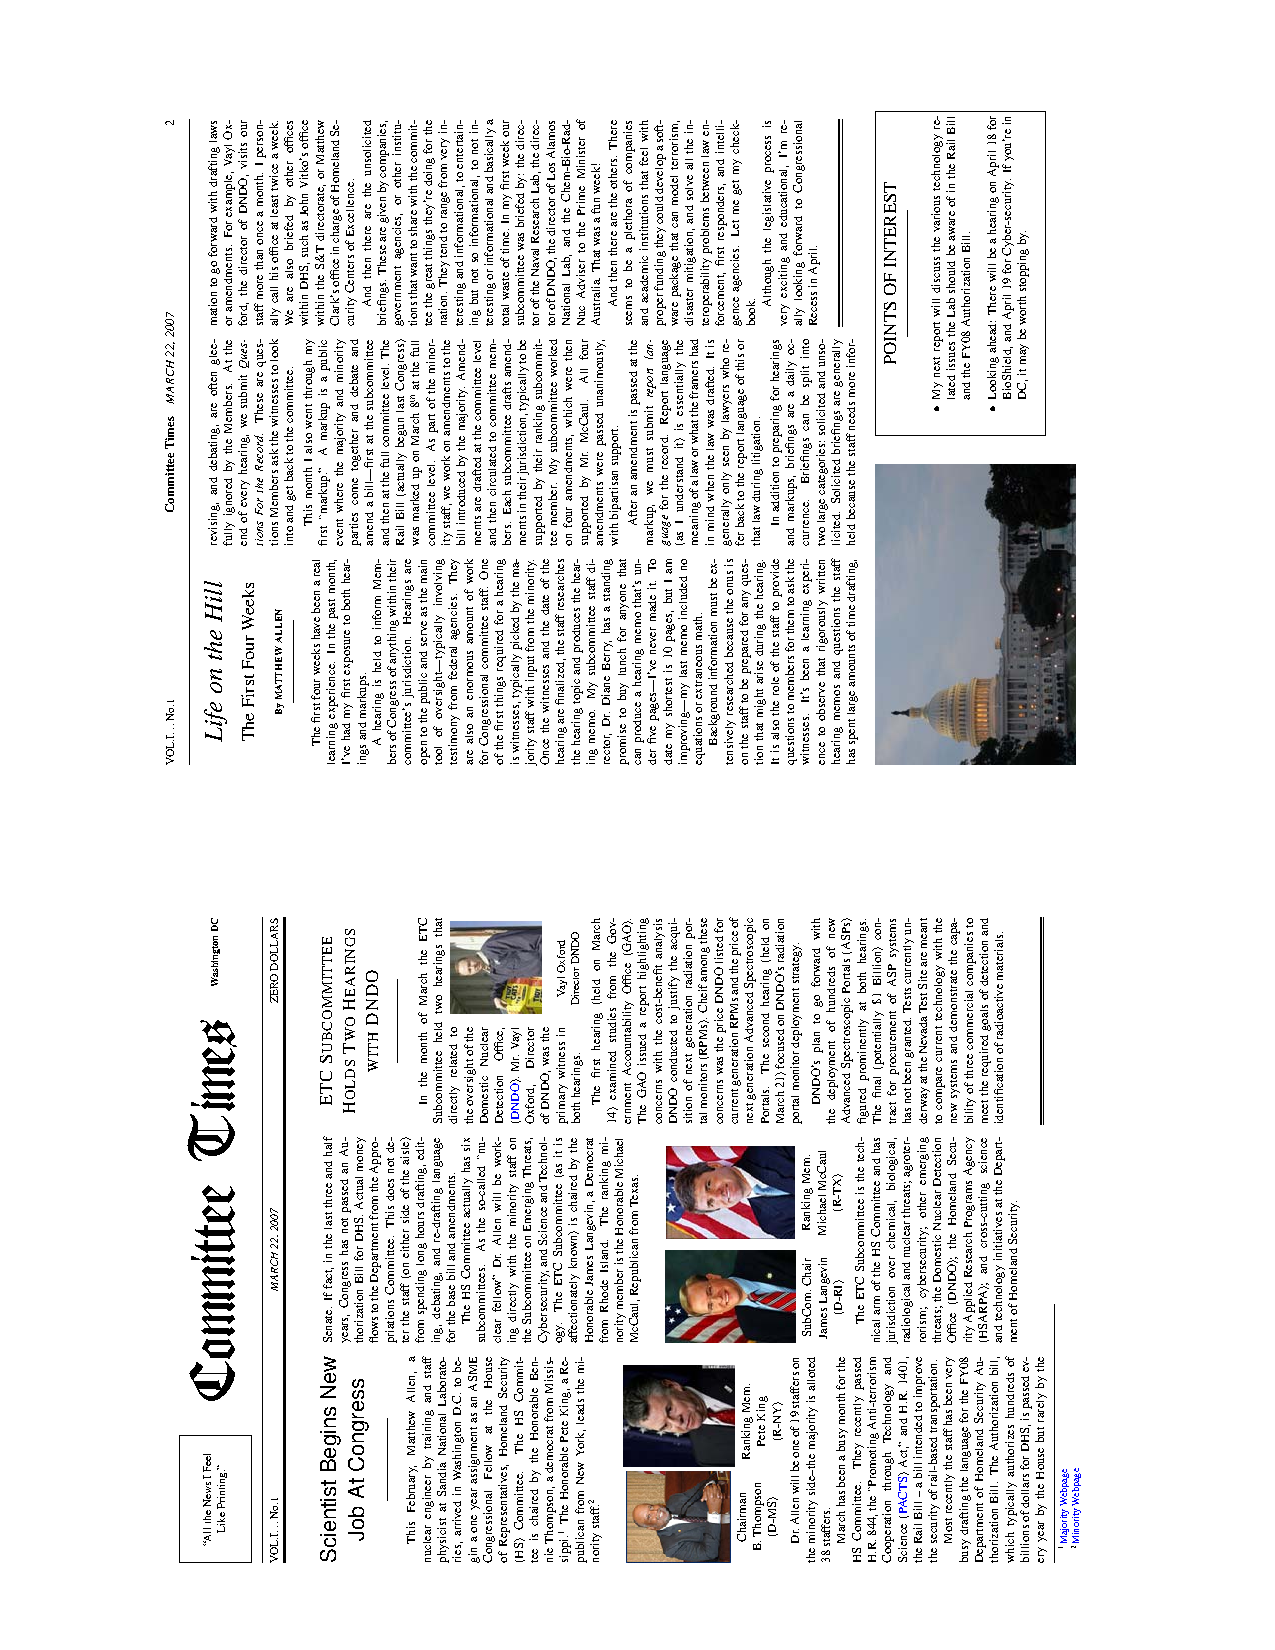
\includegraphics[width=5in]{Figure2}}
%	\end{center}
% \caption{Demonstration of the default settings used in conjunction with the 
%	\texttt{multicols} and \texttt{picinpar} packages.}
% \label{fig:example}
% \end{figure}
%	\end{landscape}
% 
% \subsection{Newspaper Macros}
% 
%  The package provides a few macros that help when writing articles in column format.  As seen in Figure~\ref{fig:example}, I typically used a three column format, but these commands also work for any size column.
% 
%  The |\headline|\marg{text} command is used \DescribeMacro{\headline} to set the headline of the article. It's a good idea to use different style headlines for each article.  This helps the reader distinguish between different topics.  As you can see from Figure~\ref{fig:example}, I have used several different styles for the three articles I produced.  
%
%  Using the above two commands the articles shown in Figure~\ref{fig:example} would be set with the following commands:
% \begin{quote}
% |\headline{\bf\sf\LARGE Scientist Begins New Job At Congress}|\\
% \meta{body of the article}\\
% |\closearticle|\\[12pt]
% |\headline{\sc\Large ETC Subcommittee Holds Two Hearings with DNDO}|\\
% \meta{body of the article}\\
% |\closearticle|\\[12pt]
% \end{quote} 
%
% When writing an editorial or if you just want to add a by-line, use the |\byline| \DescribeMacro{\byline} command.  This command works in almost the same way as |\headline|, but has an additional argument for the author credit.  The author name is set in all uppercase letters after the word ``By'' directly under the article headline.  The command is called by
% \begin{quote}
% |\byline|\marg{headline}\marg{author}
% \end{quote}
% where \marg{headline} is the title of the article and \marg{author} is the name you would like to appear under that title.
%
% If you want to add a subtitle before the The headline/byline combination as shown on the second page of Figure~\ref{fig:example}, you have to play with the spacing a little bit.  The command used in the example is:
% \begin{quote}
% |\byline{{\it\huge Life on the Hill}\\[10pt]|\\
% \hspace*{1.0in}|{\Large The First Four Weeks}\\[10pt]}{Matthew Allen}|
% \end{quote}
% Someday I may go back and add a |\subtitle| command, but for now I just play with the spacing manually.
%
% The |\closearticle| command \DescribeMacro{\closearticle} is used to show the end of an article.  This command produces a small double-line rule the width of the column.  It is useful when an article ends in the middle of column, before you declare the next headline.  The |\closearticle| command does contain the parameter |\hsize|, which is the value of column width used by the \textsf{multicols} package .  If you're not using the \textsf{multicols} package, this command could produce an error.
%
% \section{Implementation}
%
% \StopEventually{\PrintChanges}
% Here we load the only \emph{required} package.

%    \begin{macrocode}
%%%%%% 	Package Loading   %%%%%%
\RequirePackage{yfonts}  % used for the paper title font

%    \end{macrocode}
% Next we have the main body of the code, and begin by defining the font used for the Headline.
%    \begin{macrocode}

%%  Define font for page title  %%
\DeclareFontFamily{T1}{bigygoth}{}
\DeclareFontShape{T1}{bigygoth}{m}{n}{<->s*[2.5]ygoth}{}
%    \end{macrocode}
%	Next we set up the page dimensions.  We could have used the \textsf{geometry} package here, but I like to avoid loading packages when I can.  The default values for the \texttt{article} class are shown to the right of the length commands.
%    \begin{macrocode}

%%%%%%%%%%% Define Text Dimensions  %%%%%%%
\setlength\topmargin{-48pt} 		% article default = -58pt
\setlength\headheight{0pt}  		% article default = 12pt
\setlength\headsep{34pt}		% article default = 25pt
\setlength\marginparwidth{-20pt}	% article default = 121pt
\setlength\textwidth{7.0in}		% article default = 418pt
\setlength\textheight{9.5in}		% article default = 296pt
\setlength\oddsidemargin{-30pt}
%    \end{macrocode}
%	\begin{macro}{\currentvolume}
%	\begin{macro}{\currentissue}
%	Define the volume and issue number.  These values must be entered manually.
%    \begin{macrocode}

%%%% counters for volume and number %%%%
\newcounter{volume}
\newcommand\currentvolume[1]{\setcounter{volume}{#1}}
\newcounter{issue}
\newcommand\currentissue[1]{\setcounter{issue}{#1}}
%    \end{macrocode}
%	\end{macro}
%	\end{macro}
% \begin{macro}{\@papername}
% \begin{macro}{\@headername}
% \begin{macro}{\@paperlocation}
% \begin{macro}{\@paperslogan}
% \begin{macro}{\@paperprice}
% Set up the package defaults
%    \begin{macrocode}

%%%% set internal variables %%%%
\def\@papername{Committee Times:}
\def\@headername{Committee Times}   
\def\@paperlocation{Washington DC}
\def\@paperslogan{``All the News I Feel Like Printing.''}
\def\@paperprice{Zero Dollars}
%    \end{macrocode}
% \end{macro}
% \end{macro}
% \end{macro}
% \end{macro}
% \end{macro}
% \begin{macro}{\SetPaperName}
% \begin{macro}{\SetHeaderName}
% \begin{macro}{\SetPaperLocation}
% \begin{macro}{\SetPaperSlogan}
% \begin{macro}{\SetPaperPrice}
% Set up the commands to modify the behavior.
%    \begin{macrocode}

\newcommand\SetPaperName[1]{%
	\def\@papername{#1}}
\newcommand\SetHeaderName[1]{%
	\def\@headername{#1}}
\newcommand\SetPaperLocation[1]{%
	\def\@paperlocation{#1}}
\newcommand\SetPaperSlogan[1]{%
	\def\@paperslogan{#1}}
\newcommand\SetPaperPrice[1]{%
	\def\@paperprice{#1}}
%    \end{macrocode}
% \end{macro}
% \end{macro}
% \end{macro}
% \end{macro}
% \end{macro}
% \begin{macro}{\maketitle}
% Redefine the |\maketitle| command.  This is only for the first page.
%    \begin{macrocode}

%%%%%%%%%%% Redefine \maketitle     %%%%%%%
\renewcommand{\maketitle}{\thispagestyle{empty}
\vspace*{-40pt}
\begin{center}
{\setlength\fboxsep{3mm}\raisebox{12pt}{\framebox[1.2\width]{\parbox[c]{1.15in}{\begin{center}\small \@paperslogan\end{center}}}}}\hfill%
{\textgoth{\huge\usefont{T1}{bigygoth}{m}{n} \@papername}}\hfill%	
\raisebox{12pt}{\textbf{\footnotesize \@paperlocation}}\\
\vspace*{0.1in}
\rule[0pt]{\textwidth}{0.5pt}\\
{\small VOL.\MakeUppercase{\roman{volume}}\ldots No.\arabic{issue}} \hfill \MakeUppercase{\small\it\@date} \hfill {\small\MakeUppercase{\@paperprice}}\\
\rule[6pt]{\textwidth}{1.2pt}
\end{center}
\pagestyle{plain}
}
%    \end{macrocode}
% \end{macro}
% At this point we redefine the pape style for all subsequent pages.  
%    \begin{macrocode}

%%%%%%%   redefine plain page style  %%%%%%%
\renewcommand{\ps@plain}{%
		\renewcommand\@oddfoot{}%					% empty recto footer
		\let\@evenfoot\@oddfoot						% empty verso footer
		\renewcommand\@evenhead
			{\parbox{\textwidth}{\vspace*{4pt}
			{\small VOL.\MakeUppercase{\roman{volume}}\ldots No.\arabic{issue}}\hfill\normalfont\textbf{\@headername}\quad\MakeUppercase{\it\@date}\hfill\textrm{\thepage}\\
			\rule{\textwidth}{0.5pt}
			\vspace*{12pt}}}%
		\let\@oddhead\@evenhead}
%    \end{macrocode}
% \begin{macro}{\headline}
% \begin{macro}{\byline}
% \begin{macro}{\closearticle}
% Define the |\headline| and the |\byline| commands.  The |\closearticle| command is intended to be used at the conclusion of each article.
%    \begin{macrocode}

%%%%%%%%%%%  Headline (with byline) command  %%%%%%%%%
\newcommand\headline[1]{\begin{center} #1\\ %
			\rule[3pt]{0.4\hsize}{0.5pt}\\ \end{center} \par}
\newcommand\byline[2]{\begin{center} #1 \\%
			{\footnotesize\bf By \MakeUppercase{#2}} \\ %
			\rule[3pt]{0.4\hsize}{0.5pt}\\ \end{center} \par}
\newcommand\closearticle{{\begin{center}\rule[6pt]{\hsize}{1pt}\vspace*{-16pt}
			\rule{\hsize}{0.5pt}\end{center}}}
%%%%%%%%%%%%%%%%%%%% End of Package   %%%%%%%%%%%%%%%
%    \end{macrocode}
% \end{macro}
% \end{macro}
% \end{macro}
% \Finale



